\documentclass[12pt]{article}
\usepackage[toc,page]{appendix}
\usepackage{amsmath}
\usepackage{amsfonts}
\usepackage{graphicx}
\usepackage{url}
\usepackage{cite}
\title{jahmm: a tool for discretizing multiple ChIP-seq profiles}
\author{Guillaume Filion and Pol Cusc\'o}

\begin{document}
\maketitle

\section{Abstract}
Chromatin immunoprecipitation and high throughput sequencing (ChIP-seq) is the \textit{de facto} standard method to map chromatin features on genomes. The output of ChIP-seq is quantitative within a single genome-wide profile, but there is no natural way to compare experiments, which is why the data is often discretized as present/absent calls. Many tools perform this task efficiently, however they process a single input at a time, which produces discretization conflicts among replicates. Here we present the implementation of a Hidden Markov Model (HMM) using mixture negative multinomial emissions to discretize ChIP-seq profiles. The method gives meaningful discretization for a wide range of features and allows to merge datasets from different origins into a single discretized profile, which resolves discretization conflicts. A quality control step performed after the discretization accepts or rejects the discretization as a whole. The implementation of the model is called jahmm, and it is available as an R package. The source can be downloaded from \url{http://github.com/gui11aume/jahmm}.



\section{Introduction}
The discovery that genes are activated and repressed by transcription factors (proteins that regulate transcription) was the foundation of the modern theory of gene regulation \cite{pmid15950866}. More recent work on histone post-translational modifications (PTMs) showed that they play a key role in the regulation of transcription. However, the influence of transcription factors and histone PTMs on transcription is still poorly understood, in part because of the discrepancy between their behavior \textit{in vivo} and \textit{in vitro}.

Chromatin immunoprecipitation (ChIP) was the first method to address the need to analyze protein-DNA interactions in the context of the nucleus \cite{pmid2454748}. Earlier methods such as footprinting and electrophoretic mobility shift assays were invaluable in their time, but they could not guarantee that a protein of interest was present on a given sequence of the genome \textit{in vivo}. The advent of microarrays and later high throughput sequencing gave genome-wide insight into the distribution of transcription factors, but these technologies raised several statistical issues that are still not resolved today. Such methods produce a large amount of data (currently of the order of 100 million reads per run), which calls for efficient and robust analysis methods.

The constant improvement of high throughput sequencing technologies makes the comparison of experiments performed at different dates inconvenient. In addition, it is practically impossible for two laboratories to produce identical ChIP-seq results due to the high number of steps and the complexity of the protocol. For these reasons, the classical approach is to discretize ChIP-seq signals to obtain a call specifying whether the feature of interest is present or absent at every position of the genome. This process is often referred-to as ``peak finding'' in the biological literature, because transcription factors are believed to bind a single location in a large neighborhood. In practice however, ChIP-seq signals (histone PTMs in particular) often consist of wide domains extending over several Kb.

Many peak finding tools have been developed since the emergence of the ChIP-seq technology, the most popular of which are PeakFinder \cite{pmid17540862}, FindPeaks \cite{pmid18599518}, CisGenome \cite{pmid18978777}, MACS \cite{pmid18798982}, SISSRs \cite{pmid18684996}, BayesPeak \cite{pmid19772557} and HPeak \cite{pmid20598134}. BayesPeak and HPeak are based on elaborate statistical models accounting for the overdispersion of ChIP-seq signals and implement a Hidden Markov Model (HMM). However, all these tools can discretize only one ChIP-seq profile at a time, which creates call conflicts when replicates are available. The IDR (Irreproducible Discovery Rate \cite{li2011}) is an endeavour to solve this issue, but it is restricted to two replicates, meaning that there is no solution for conflict resolution when more than two replicates are available.

Here we present a model addressing this issue. The jahmm (Just Another HMM) discretizer uses an HMM with mixture negative multinomial emissions. This distribution is a good representation of the sequence count at the output of modern sequencers, and it offers an intuitive interpretation as Gamma-Poisson process. The jahmm discretizer not only allows to discretize any ChIP-seq profile, it also allows to combine signals from different sources and/or different technologies into a single discretized profile. Finally, jahmm includes an atomic quality control step that either accepts the discretization or rejects it as a whole.

\section{Results}

Here we present an accessible overview of jahmm. Mathematical details and complements can be found in the annexes.

\subsection{Motivation for the emission model}

At the output of a ChIP-seq experiment, we assume that the genome is segmented in windows of identical size and that reads from the sequencer are mapped on the genome and binned in those windows. The number of reads mapping to a genomic window is a discrete variable without upper limit, so the Poisson distribution comes as a natural first guess. However, this choice imposes that the mean number of reads is equal to the variance, which poorly matches experimental observations. It is indeed well known that the distribution of read counts in ChIP-seq experiments is overdispersed \cite{pmid19772557,pmid20598134}.

Fig. 1a shows  the read count distribution in an experiment performed without immunoprecipitation (the DNA is broken by sonication and sequenced), which describes the baseline distribution of ChIP-seq signals for 300 bp windows. The red histogram shows the distribution of a Poisson variable fitted to the observation. The variance of the observed distribution is more than 3 times larger than the mean and the difference between these distributions is evident for low read counts. For larger windows, the lack of fit of the Poisson distribution becomes more pronounced, as shown in Fig. 1b (in this case the variance is more than 10 times larger than the mean). Discarding non mappable windows reduces the skew but the resulting distribution is not Poisson (data not shown). In summary, the Poisson distribution is not suitable to model ChIP-seq experiments.

\begin{figure}
  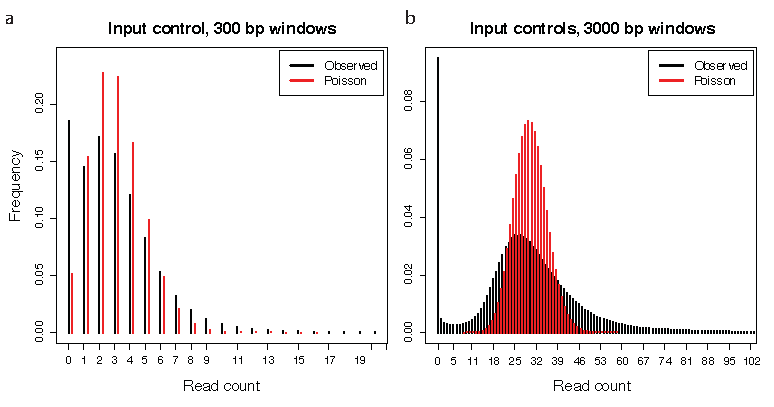
\includegraphics[width=\textwidth]{Fig1.pdf}
  \caption{ChIP-seq read count distribution.
  Left (\textbf{a}): distribution of read counts for a negative control
  experiment in 300 bp windows (black bars) and the corresponding fitted
  Poisson distribution (red bars). Notice the lack of fit for the number
  of windows with no read and for windows with 7 and higher reads.
  Right (\textbf{b}): same as \textbf{a} for 3000 bp windows.}
\end{figure}

The negative binomial distribution is more flexibile because it has two parameters, which allows to separate the mean from the variance. More importantly, an intuition of this distribution is given by the two step ``Gamma-Poisson mixture''. In the first step, a parameter $\lambda$ is drawn from a Gamma distribution; in the second step, a random observation is drawn from a Poisson distribution with parameter $\lambda$. In other words, the negative binomial distribution can be viewed as a mixture of Poisson distributions with means (\textit{i.e.} $\lambda$ parameters) distributed as a Gamma random variable.

In the case of ChIP-seq experiments, the mean number of reads mapping to a window is expected to vary due to experimental and computational biases. The G+C content is known to affect the efficiency of the PCR amplification taking place before sequencing. As a consequence, the number of reads is expected to depend on the G+C content of the window. In addition, read mappability is not constant throughout the genome because of polymorphism and repeated sequences, which can decrease the number of mappable reads. These variations are not expected to have an exact Gamma distribution, but since the shape of the Gamma family is flexible, it is a good approximation for many unimodal distributions.

However, the read distribution is clearly bimodal for large windows (Fig. 1b) and is skewed for smaller windows (Fig. 1a). This bimodality is mostly due to the repeated sequences of the genome, since mapping the human genome sequence (hg19) onto itself without any experimental step yields a multimodal distribution (not shown). A mixture of two negative binomial distributions was thus chosen to model the amount of read counts mapping to each genomic window. The mixture model can be estimated efficiently with the EM algorithm \cite{Dempster77maximumlikelihood} and gives a good fit for short windows (Fig. 2a). For 3000 bp windows, the central part of the distribution shows a misfit, but the tails are well captured by the model, which makes it robust to overdispersion. Fitting the right tail is a key property for a discretization model because it reduces the number of false positives compared to the Poisson distribution.

\begin{figure}
  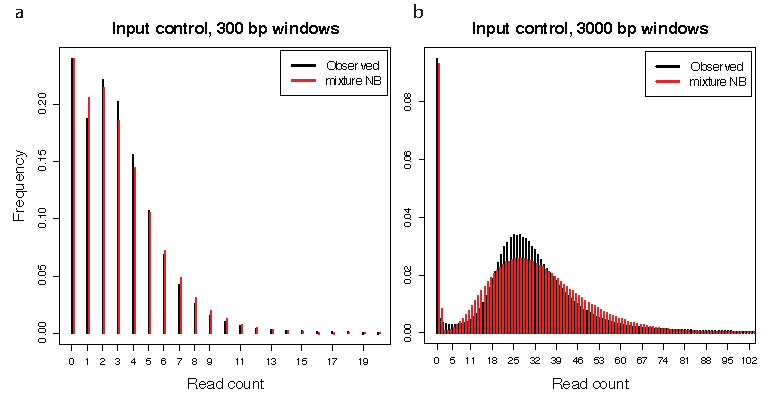
\includegraphics[width=\textwidth]{Fig2.pdf}
  \caption{Fit of the mixture negative binomial model.
  Left (\textbf{a}): same as Fig. 1a, but the red bars represent the corresponding
  negative binomial mixture distribution fitted by the EM algorithm.
  Right (\textbf{b}): same as \textbf{a} for 3000 bp windows. The mixture negative
  binomial model is a good fit for the tail of the distribution.}
\end{figure}

%The bimodality of the distribution suggests that genomic windows belong to either the high or low mappability class. We will follow this interpretation throughout, and we will further assume that these classes differ in the ``scale'' parameter of the underlying Gamma-Poisson process.

\subsection{Implementation and test}
The input of jahmm consists of a set of binned ChIP-seq profiles (assumed to be replicates of each other) plus one negative control ChIP-seq profile binned in the same way. This profile is instrumental to estimate the baseline variations of the read count per window.
The output is a single profile of present/absent calls per genomic window. Each ChIP-seq profile represents one dimension of the emissions, modelled by the mixture negative binomial distribution motivated above. We assume that the ``shape'' parameter of the Gamma distribution underlying the Gamma-Poisson process is a global parameter fixed by the genome and the window size. This means that every genomic window is associated to a reference $\lambda$ parameter, and that the number of reads in each profile have a Poisson distribution with a fixed scaling relative to the reference. These assumptions make the profiles a mixture of negative multinomial variables.

The HMM is assumed to have 3 states, only one of which is interpreted as ``present'' or ``target''; the other 2 are interpreted as ``absent''. Hands-on experience with ChIP-seq data shows that many profiles consist of 3 distinct levels (typically ``depleted'', ``average'', ``enriched'') and that low-frequency baseline variations can sometimes capture one state of the HMM, which masks the highest peaks. For these reasons a 3-state model is more robust to process vastly different ChIP-seq data. The full model is fitted using the Baum-Welch algorithm \cite{baum1966}, followed by a multi-thread variant of simulated annealing \cite{pmid17813860} to reduce the chances of being trapped in a local optimum. The present/absent calls are then attributed to each window using the Viterbi algorithm \cite{1054010}, which returns the optimal segmentation under the observations and the fitted model.

Finally, a quality control (QC) for the segmentation is performed using the smoothing distribution of the HMM (the posterior distribution of the states given the emissions). The QC score is the estimated probability of false positives among the ``present'' calls, which expresses the confidence of the classifier for these calls. In the negative controls we have tested (profiles containing no target), the estimated false positive rate is higher than 0.09 for 300 bp windows. The QC is atomic, in other words the discretization is rejected altogether if the QC score of the sample exceeds this threshold value. Because there are high confidence peaks even in negative controls, it is more meaningful to judge the validity of the discretization, rather than the reliability of each call.

We used jahmm on ENCODE ChIP-seq data \cite{pmid22955991} for the transcription factor CTCF which is known to bind its targets as single peaks, and for the histone PTM H3K27me3 which is known to be present in the genome in domains. The datasets were produced from the K562 myelogenous leukaemia cell line by different laboratories (five distinct laboratories for CTCF and three for H3K27me3). Fig. 3a and 3b shows that the discretization closely matches the visual expectations in both cases, which is supported by the fact that the QC scores are below the rejection threshold (0.015 and 0.057 respectively).


\begin{figure}
  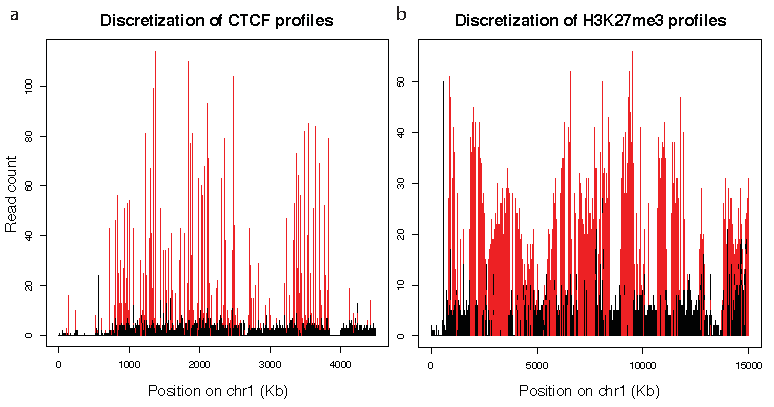
\includegraphics[width=\textwidth]{Fig3.pdf}
  \caption{Example discretization by jahmm.
  Left (\textbf{a}): Discretization of CTCF binding sites. For concision
  only one of the thirteen profiles used for the discretization is shown.
  The ``present'' calls are indicated in red.
  Right (\textbf{b}): Riscretization of H3K27me3 domains.
  As for \textbf{a}, only one of the five profiles used for the discretization
  is shown with the same color code. Notice the different scale of the x axis
  in both panels.}
\end{figure}

We also used jahmm to discretize profiles of HDAC6 from a single laboratory. HDAC6 has an overwhelmingly cytosolic distribution \cite{pmid12024216}, it should therefore give a baseline signal with no target. In this case, the discretization proceeded normally, but the QC score was 0.17, exceeding the threshold. This suggests that the discretization of this profile is meaningless. Therefore jahmm can be used to discretize ChIP-seq signals of different types, without prior knowledge of the signal under study, nor of the quality of the experiment.

\section{Methods}
\subsection{ChIP-seq data processing}
The raw data .fastq files linked in the supplementary file \texttt{downloads.lst} were downloaded from the ENCODE repository.

Mapping was carried out by gem \cite{pmid23103880} with options \texttt{-q ignore -m 2 -T 4 --unique mapping}. The versions of gem-indexer and gem-mapper were 1.423 (beta), and 1.376 (beta) respectively. The
sequence of the human genome (hg19) in fasta format was downloaded from \url{http://hgdownload.cse.ucsc.edu/goldenPath/hg19/bigZips/chromFaMasked.tar.gz}.


%% REFERENCES %%
\bibliography{references}{}
\bibliographystyle{plain}


%%%%%%%%%%%%%%%%%%%%%%%%%%%%%%%%%%%%%%%%%%%%%%%%%%%%
%%               Technical appendix               %%
%%%%%%%%%%%%%%%%%%%%%%%%%%%%%%%%%%%%%%%%%%%%%%%%%%%%


\newpage
\begin{appendices}


%In the text, we often refer to the gamma and polygamma functions.
%Euler's $\Gamma$ function is defined as
%$\Gamma(\alpha) = \int_0^{\infty}t^{\alpha+1}e^{-t}dt$.
%The digamma function, noted $\psi(\alpha)$ is the
%derivative of $\log \Gamma(\alpha)$, and the trigramma function,
%noted $\psi'(\alpha)$ is the derivative of the digamma function.

We start with some generalities about Hidden Markov Models and then
derive a model targeted to ChIP experiments with replicates.

\section{Hidden Markov Models}

    We will consider only discrete Hidden Markov models (HMMs) and
    will simply refer to them as Hidden Markov model, without mention
    of the term `discrete' for simplicity.  HMMs are defined by

    \begin{enumerate}
      \item a set $S$ of $m$ states numbered from 1 to $m$,
      \item an initial state probability distribution $\nu$, which
      gives the probabilities that the system is initially in state $i$,
      \item an $m \times m$ transition matrix $Q$ which contains the
      probabilities $Q(i,j)$ that the system goes from state $i$ to
      state $j$,
      \item $m$ distributions denoted $g_i$ $(i = 1, \ldots, m)$, which
      give the emission probabilities in the different states.
    \end{enumerate}

\subsection{The HMM formalism applied to ChIP-seq}
\label{sec:HMM_formalism}

    The output of ChIP-seq experiments consists of genomic profiles
    that can be thought of as ordered windows of equal size. Each
    window is associated to a certain number of read counts coming
    from different replicate experiments or negative controls.

    HMMs are particularly adapted to this framework. The read counts
    associated to each window can be thought of as the observable
    emissions, whereas the unobservable states can be thought of
    the possible processes ongoing on those windows. Typically, the
    states may correspond to the events ``the protein of interest
    is bound on the window'' and ``the protein of interest is not
    bound on the windown''. There may be more states, and they do
    not have to correspond to a protein binding event (most notably,
    they can correspond to the present of some histone modifications).

    The rest of this section pertains to general HMMs and will not
    make any hypothesis regarding the nature of the states and the
    emissions, however it can be useful for the intuition to think
    about states are chromatin states, and emissions as read counts.

\subsection{The Forward-Backward algorithm}

    For a sequence of emissions $y_0, \ldots, y_n$, the likelihood
    of the state sequence $i_0, \ldots, i_n$ is proportional to

    $$ \nu(i_0)g_{i_0}(y_0)
       \prod_{k=1}^n Q(i_{k-1},i_k)g_{i_k}(y_k). $$

    By summing over all possible combinations of states, we obtain
    the normalizing constant $L_n$ such that

    \begin{equation}
       L_n = \sum_{i_0 \in S, \ldots, i_n \in S} \nu(i_0)g_{i_0}(y_0)
       \prod_{k=1}^n Q(i_{k-1},i_k)g_{i_k}(y_k).
    \end{equation}

    We denote $\phi_{k|n}(i)$ the probability that the system is in
    state $i$ at time $k$ given the emissions $y_0, \ldots, y_n$. If
    we call $S_n(k,i)$ the set of $n$-tuples $(i_0, \ldots, i_n)$
    such that $i_k = i$, the value of $\phi_{k|n}(i)$ comes as

    $$ \phi_{k|n}(i) = \frac{1}{L_n}
       \sum_{(i_0, \ldots, i_n) \in S_n(k,i)}
       \nu(i_0)g_{i_0}(y_0) \prod_{l=1}^n Q(i_{l-1}, i_l)
       g_{i_l}(y_l). $$

    We now introduce $\alpha_k(i)$ the probability that the
    system is in state $i$ at time $k$ given the emissions
    $y_0, \ldots, y_k$, and the $\beta_{k|n}(\cdot)$ the numerical
    function such that $\phi_{k|n}(i) = \alpha_k(i)\beta_{k|n}(i)$.

    \begin{align*}
      \alpha_k(i) &= \frac{1}{L_k}
      \sum_{i_0=1}^m \cdots \sum_{i_{k-1}=1}^m
      \nu(i_0)g_{i_0}(y_0) \prod_{l=1}^{k-1} Q(i_{l-1},i_l) g_{i_l}(y_l)
      Q(i_{k-1}, i)g_i(y_k) \\
      \beta_{k|n}(i) &= \frac{L_k}{L_n}
      \sum_{i_{k+1}=1}^m \cdots \sum_{i_n=1}^m
      Q(i, i_{k+1})g_{i_{k+1}}(y_{k+1})
      \prod_{l=k+2}^n Q(i_{l-1}, i_l)g_{i_l}(y_l)
    \end{align*}

    To preserve the equality $\phi_{k|n}(i) = \alpha_k(i)\beta_{k|n}(i)$
    for every $k$, we set by definition $\beta_{n|n}(i) = 1$.
    From the equations above, we draw the following recursive
    equations:

    \begin{align} \alpha_k(i) &= \frac{L_{k-1}}{L_k}
      \sum_{j=1}^m \alpha_{k-1}(j) Q(j,i) g_i(y_k) \label{alpha} \\
      \beta_{k|n}(i) &= \frac{L_k}{L_{k+1}}
      \sum_{j=1}^m Q(i,j) g_j(y_{k+1})
      \beta_{k+1|n}(j). \label{beta}
    \end{align}

    Equations (\ref{alpha}) and (\ref{beta}) are the basis of the
    Forward-Backward algorithm to compute $\phi_{k|n}(i)$. The terms
    $\alpha_k(i)$ can be recursively computed from $k=0$ to $k=n$
    with equation (\ref{alpha}), and the terms $\beta_{k|n}(i)$
    can be computed from $k=n-1$ to $k=0$ with equation (\ref{beta}).
    The terms $\phi_{k|n}(i)$ are then found as the product
    $\alpha_k(i)\beta_{k|n}(i)$.

    We now turn to the term $\phi_{k-1,k|n}(i,j)$, which is by
    definition the probability that the system is in state $i$ at
    time $k-1$ and in state $j$ at time $k$ given $y_0, \ldots, y_n$.
    If we call $S_n(k,i,j)$
    the set of $n$-tuples $(i_0, \ldots, i_n)$ such that
    $i_{k-1} = i$ and $i_k = j$, we get

    \begin{align}
      \phi_{k-1,k|n}(i,j) &= \frac{1}{L_n}
       \sum_{(i_0, \ldots, i_n) \in S_n(k,i,j)}
       \nu(i_0)g_{i_0}(y_0) \prod_{l=1}^n Q(i_{l-1}, i_l)
       g_{i_l}(y_l) \nonumber \\
        &= \frac{L_{k-1}}{L_k}
       \alpha_{k-1}(i) Q(i,j) g_j(y_k) \beta_k(j). \label{phiQ}
    \end{align}

    When the $\alpha_k(i)$ and the $\beta_{k|n}(i)$ have been
    computed by the Forward-Backward algorithm, we also have access
    to the $\phi_{k-1,k|n}(i,j)$ by using formula (\ref{phiQ}).

\subsection{The Baum-Welch algorithm}
\label{sec:Baum-Welch}

    The Baum-Welch algorithm is the special case of the EM algorithm
    applied to HMMs. Let us consider the general case of the triplet
    $(X, Z, \theta)$ where the variable $X$ is observed, $Z$ is not
    observed, and $\theta$ is the set of parameters of the distribution
    of $(X,Z)$. The full likelihood $\mathcal{L}_0(X, Z, \theta)$
    cannot be computed because the value of $Z$ is unknown.

    To find the value of $\theta$ that maximizes the full likelihood,
    we introduce an iterative procedure where the values of the
    parameter are updated upon each iteration. The current value of
    $\theta$ is noted $\theta^{(t)}$, and we compute the expected
    complete log-likelihood $\mathcal{Q}(\theta|\theta^{(t)})$
    assuming the current value of $\theta$ (note the difference
    between the intermediate quantity of the EM $\mathcal{Q}$ and
    the transition matrix $Q$).

    $$ \mathcal{Q}(\theta|\theta^{(t)}) =
      E_{Z|X, \theta^{(t)}} \left\{
      \log \mathcal{L}_0(X, Z, \theta^{(t)}) \right\}$$

    This computation is called the E-step. The notations mean that
    the expectation is taken over the variable $Z$, assuming that
    it is conditional on the observed values of $X$ and that the
    parameters of the distribution are given by $\theta^{(t)}$.
    The E-step is followed by the
    M-step, in which $\theta^{(t+1)}$ is set to the value of
    $\theta$ that maximizes $\mathcal{Q}(\theta|\theta^{(t)})$.

    In the case of HMMs, the variable that is not observed is the
    sequence of states. The set of parameters $\theta^{(t)}$
    represents the transition probabilities (the matrix $Q$)
    and the parameters of the $m$ distributions of the emissions.

    The log-likelihood of the state sequence $(i_0, \ldots, i_n)$
    is

    $$ \log \nu(i_0) + \sum_{k=1}^n \log Q(i_{k-1}, i_k)
      + \sum_{k=0}^n \log g_{i_k}(i_k, \theta). $$

    The addition of $\theta$ to the terms above emphasizes that they
    depend on the value of the parameters. To compute
    $\mathcal{Q}(\theta|\theta^{(t)})$, we need to take the
    expectation of the above over the state sequence
    conditionally on $y_0, \ldots, y_n$ and assuming that the parameters
    are given by $\theta^{(t)}$.

    \begin{align}
      \mathcal{Q}(\theta|\theta^{(t)}) &=
      E_{\theta^{(t)}} \left\{ \log \nu(i_0)
      \big| y_0, \ldots, y_n \right\} + \nonumber \\
      &\sum_{k=1}^n E_{\theta^{(t)}} \left\{
        \log Q(i_{k-1}, i_k)\big| y_0,
            \ldots, y_n \right\} + \label{eq:QEM} \\
      &\sum_{k=0}^n E_{\theta^{(t)}} \left\{
        \log g_{i_k}(y_k, \theta) \big| y_0, \ldots, y_n \right\}
        \nonumber
    \end{align}

    In practice, the first term of (\ref{eq:QEM}) will often not depend
    on $\theta$ so it will not contribute to the evaluation.
    The third term can be rewritten as

    $$\sum_{k=0}^n\sum_{i=1}^m \phi_k(i) \log g_{i_k}(y_k, \theta).$$

    This term depends on the emission probabilities, and nothing
    can be said about it in general terms because they differ
    between different models. But the second term depends only on
    the transition probabilities, which are present in every HMM,
    and it can be solved in general. First we notice that

    \begin{align*}
      &E_{\theta^{(t)}} \left\{ \log Q(i_{k-1}, i_k)
      \big| y_0, \ldots, y_n \right\} = \\
      &E_{\theta^{(t)}} \left\{ \sum_{i=1}^m\sum_{j=1}^m
      1_{\{(i_{k-1}, i_k) = (i,j)\}} \log Q(i,j)
      \big| y_0, \ldots, y_n \right\} = \\
      &\sum_{i=1}^m\sum_{j=1}^m E_{\theta^{(t)}} \left\{
      1_{\{(i_{k-1}, i_k) = (i,j)\}} \big| y_0, \ldots, y_n \right\}
      \log Q(i,j)
    \end{align*}

    Remember that by definition $E_{\theta^{(t)}} \left\{
    1_{\{(i_{k-1}, i_k) = (i,j)\}} \big| y_0, \ldots, y_n \right\}$
    is $\phi_{k-1,k}(i,j)$, so that we can rewrite the second term
    of (\ref{eq:QEM}) as

    $$ \sum_{k=1}^n\sum_{i=1}^m\sum_{j=1}^m \phi_{k-1,k}(i,j)
      \log Q(i,j). $$

    The values of $\phi_{k-1,k}(i,j)$ are computed during the
    E-step by the Forward-Backward algorithm.
    The terms $Q(i,j)$ are part of $\theta$ and are thus updated
    during the M-step. By using Lagrange multipliers, we can show
    that the update values are

    $$ Q(i,j)^{(t+1)} = \frac{\sum_{k=1}^n \phi_{k-1,k}(i,j)}
      {\sum_{k=1}^n\sum_{l=1}^m\phi_{k-1,k}(i,l)}. $$

    To complete the Baum-Welch algorithm, we need to compute the last
    term of (\ref{eq:QEM}), which requires making a model for the
    emissions.

\section{Zero-Inflated Negative Multinomial}
\label{sec:nb}

The Baum-Welch algorithm provides a general framework to estimate
the transition probabilities and the emission parameters. However,
the detail of the estimation depends on the emission model. Here
we give some general results about the negative multinomial and
the zero-inflated negative multinomial distributions that will
be useful to setup a model for emissions in ChIP-seq experiments.

\subsection{The Gamma-Poisson process}
\label{sec:gamma_poisson}

    The Gamma-Poisson process can describe many phenomena
    because of the flexibility of the Gamma distribution. The
    $\alpha$ parameter of the Gamma distribution is often referred
    to as the ``shape'' parameter. For negative values of $\alpha$,
    the distribution has a singularity at 0, whereas for positive
    values, the distribution has a single ``bump''. The $\beta$
    parameter is often referred to as the ``scale'' parameter
    because it represents a stretching of the curve along the x-axis
    that can fit different variances. As a result, the Gamma
    distribution is a good choice for almost every continuous
    distribution with positive values and a single mode. Combined
    to the Poisson distribution, it allows to fit almost every
    discrete distribution with positive values.
    In what follows, $y$ is a non negative integer (an element of
    $\mathbb{N}$). Let $Y$ be a discrete random variable distributed
    as a Poisson distribution with parameter $\lambda$. The
    probability that $Y$ is equal to $y$ is by definition

    \begin{equation}
\label{eq:poisson}
      P(Y=y) = e^{-\lambda} \frac{\lambda^y}{y!}.
    \end{equation}

    Let us now assume that $\lambda$ is itself a random variable,
    such that the above equality is actually $P(Y=y | \lambda)$.
    If $\lambda$ is independent of $Y$ and has a Gamma distribution
    with parameters $\alpha$ and $\beta$, the joint distribution of
    $Y$ and $\lambda$ is the product of the two distributions, that
    is

    $$ e^{-\lambda} \frac{\lambda^y}{y!}
         \frac{1}{\Gamma(\alpha)\beta^{\alpha}} e^{-\lambda/\beta}
         \lambda^{\alpha-1}. $$


    The marginal distribution of $Y$, \textit{i.e.} $P(Y=y)$, is found
    by integrating the equality above over $\lambda$.

    \begin{align}
\label{eq:nb_distrib_w_beta}
      P(Y=y) &= \frac{1}{\Gamma(\alpha)\beta^{\alpha}y!}
         \int_0^{+\infty} e^{-\lambda(1+1/\beta)} \lambda^{\alpha+y-1}
         d\lambda \nonumber \\
        &= \frac{\Gamma(\alpha+y)}{\Gamma(\alpha)\beta^{\alpha}
          (1+1/\beta)^{\alpha+y} y!} \nonumber \\
        &= \frac{\Gamma(\alpha+y)}{\Gamma(\alpha)y!}
          \left(\frac{1}{1+\beta}\right)^{\alpha}
          \left(\frac{\beta}{1+\beta}\right)^y.
    \end{align}

    Equation (\ref{eq:nb_distrib_w_beta}) is the expression
    of the negative binomial distribution. If we interpret
    $p_0 = \frac{1}{1+\beta}$ and $p_1 = \frac{\beta}{1+\beta}$
    as probabilities of mutually exclusive events, we obtain the
    alternative parametrization

    \begin{equation}
\label{eq:nb_distrib}
        P(Y=y) = \frac{\Gamma(\alpha+y)}{\Gamma(\alpha)y!}
          p_0^{\alpha} p_1^y.
    \end{equation}

    In R, the \texttt{nbinom} family of functions use a
    $(\alpha, p_0)$ parametrization, but dropping $p_0$ instead
    of $p_1$ is more convenient when there are more variables
    (see section \ref{section:nm} below), so we will refer to it
    as the negative binomial disribution with parameters
    $(\alpha, p_1)$.


\subsection{The negative multinomial distribution}
\label{section:nm}

    We now introduce the case of $r$ Poisson variables that are
    conditionally independent given $\lambda$. Intuitively, this
    means that $\lambda$ is drawn at random first, which sets the
    parameter of the $r$ Poisson distributions; the Poisson
    variables are then drawn from their respective distribution
    independently of each other. In other words, the conditional
    distribution can be written as follows

    \begin{equation}
\label{eq:conditional_nm}
      P(Y_1=y_1, \ldots, Y_r=y_r|\lambda) =
      e^{-\gamma_1\lambda}\frac{(\gamma_1\lambda)^{y_1}}{y_1!}
      \ldots
      e^{-\gamma_r\lambda}\frac{(\gamma_r\lambda)^{y_r}}{y_r!}.
    \end{equation}

    Multiplying by the density of $\lambda$ and integrating as
    above, the marginal distribution of the vector
    $(Y_1, \ldots, Y_r)$ comes as

    \begin{align}
\label{eq:nm_distrib}
      P(Y_1=y_1, \ldots, Y_r=y_r) &=
      \frac{\Gamma(\alpha+y_1+\ldots+y_r)}
      {\Gamma(\alpha)y_1!\ldots y_r!}p_0^{\alpha}p_1^{y_1}
      \ldots p_r^{y_r}, \; \text{where}                \\
      p_0 &= \frac{1/\beta}{1/\beta+\gamma_1+\ldots+\gamma_r},
      \; \text{and} \nonumber \\
      p_i &= \frac{\gamma_i}{1/\beta+\gamma_1+\ldots+\gamma_r},
      \; \text{for} \; i = 1, \ldots, r. \nonumber
    \end{align}

    This distribution is called the negative multinomial, which
    the negative binomial is a special case of (for $r=1$). We will
    refer to it is as a negative multinomial with parameters
    $(\alpha, p_1, \ldots, p_r)$. It can be interpreted as the
    observations of a Gamma-Poisson process, where a common $\lambda$
    is drawn from a Gamma distribution, and $r$ variables are drawn
    from independent Poisson distributions with parameters
    $\gamma_i \lambda$ $(1 \leq i \leq r)$. The variables
    $Y_1, \ldots, Y_r$ are independent contionally on $\lambda$,
    but in section \ref{sec:marginal_nm} we prove
    that they are never unconditionally independent.

    The negative multinomial distribution has an alternative
    interpretation that sometimes proves useful. Suppose an urn
    contains black balls and balls of $r$ different
    colors in respective proportions $p_0, p_1, \ldots, p_r$, such
    that $p_0 + p_1 + \ldots + p_r =1$. If we draw balls with
    replacement from the urn until a black ball is drawn for the
    $k$-th time, the probability that the counts for the balls of
    each color are $(y_1, \ldots, y_r)$ is

    \begin{equation*}
    {k-1+y_1+\ldots+y_r \choose (k-1), y_1, \ldots, y_r}
      p_0^k p_1^{y_1} \ldots p_r^{y_r} =
    \frac{\Gamma(k+y_1+\ldots+y_r)}{\Gamma(k)y_1! \ldots y_r!}
      p_0^k p_1^{y_1} \ldots p_r^{y_r}.
    \end{equation*}

    This is formula (\ref{eq:nm_distrib}), where $\alpha$ has
    been replaced by $k$. The negative multinomial distribution is
    thus a generalization of the drawing process described above.
    From the ball and urn interpretation, we get that the observed
    counts $(y_1, \ldots, y_r)$ are twice smaller for a twice larger
    value of $p_0$ or for a twice smaller value of $\alpha$.

\subsection{Marginal distributions}
\label{sec:marginal_nm}

    To compute the marginal distributions of
    $(Y_1, \ldots, Y_r)$, we could sum over (\ref{eq:nm_distrib}),
    but it is simpler to sum over (\ref{eq:conditional_nm}) and then
    multiply by the density of $\lambda$ and integrate. The sum of
    (\ref{eq:conditional_nm}) over all indices distinct from
    $s \leq r$ is a Poisson term of the form of (\ref{eq:poisson})
    therefore, integrating over $\lambda$ yields an expression
    similar to (\ref{eq:nb_distrib}), namely

    \begin{align*}
    P(Y_s = y) &= \frac{\Gamma(\alpha+y)}{\Gamma(\alpha)y!}
      p_0^{*\alpha} p_s^{*y}, \; \text{where} \\
    p_0^* &= \frac{1/\beta}{1/\beta + \gamma_s}, \; \text{and} \\
    p_s^* &= \frac{\gamma_i}{1/\beta + \gamma_s}.
    \end{align*}

    Not surprisingly, we obtain a negative binomial distribution.
    More interestingly though, the parameters of this
    distribution are linked to the previous parameters
    by the equality $p_s^* / p_0^* = p_s / p_0$. This equality
    comes in handy to recompute the parameters of the negative
    multinomial distribution when variables are added or removed.

    In the light of the analogy with balls in an urn, this result
    is not surprising. The marginal distribution corresponds to
    the same process where some colors are removed. The proportion
    of the remaining colors change, but their relative ratios do
    not.

    To illustrate the use of this equality, we show with $r=2$ that
    the marginal variables of a negative multinomial distribution
    are never independent. This also holds for $r > 2$, which can be
    proved by induction from the observation that mutual independence
    entails pairwise independence.

    Assume that $(Y_1,Y_2)$ has a negative multinomial distribution
    and that it is not degenerate (all the parameters are strictly
    positive).  Let us fix $y_2 = 0$. The terms
    $P(y_1 = k, y_2 = 0)$ are proportional to
    $\Gamma(\alpha+k) p_1^k/k!$ and the terms $P(y_1 = k)P(y_2 = 0)$
    are proportional to $\Gamma(\alpha+k) p_1^{*k}/k!$ where
    $p_1^* = p_1 / (p_1 + p_0) < p_1$ so equality cannot hold
    for every $k \geq 0$. In conclusion, the joint distribution
    cannot be equal to the product of the marginal distributions.

    Note that the proof above assumes $p_0 > 0$, which is
    a consequence of $\beta < \infty$. So as long as $\lambda$ is
    distributed according to a proper Gamma distribution, which
    is a defining feature of the negative multinomial distribution, the
    variables cannot be independent.

    From the marginal distributions we can compute the conditional
    distribution of $(Y_1, \ldots, Y_s)$ given $(Y_{s+1}, \ldots, Y_r)$
    (and similary the distribution of any set of variables given
    the complentary set). Using the same approach as above, the
    marginal distribution is a negative multinomial that can be
    found to be

    \begin{align*}
    P(Y_{s+1}=y_{s+1}, \ldots, Y_r=y_r) &= \\
      \frac{\Gamma(\alpha + y_{s+1} + \ldots + y_r)}
      {\Gamma(\alpha)y_{s+1}! \ldots y_r!} &p_0^{\alpha}p_{s+1}^{y_{s+1}}
      \ldots p_r^{y_r} \left(\frac{1}{p_0 + p_{s+1} + \ldots + p_r}
      \right)^{\alpha+y_{s+1} + \ldots + y_r}.
    \end{align*}

    The conditional distribution is computed as the ratio of the
    full distribution and the marginal distribution.

    \begin{align*}
      P(Y_1=y_1, \ldots, Y_s=y_s|Y_{s+1}=y_{s+1}, \ldots, Y_r=y_r) &= \\
      \frac{\Gamma(\alpha + y_1 + \ldots + y_r)}
      {\Gamma(\alpha+y_{s+1}+\ldots+y_r)y_1! \ldots y_s!}
      &q_0^{\alpha+y_{s+1}+\ldots+y_r}p_1^{y_1} \ldots p_i^{y_s},
    \end{align*}

    \noindent
    where we define
    $q_0 = p_0+p_{s+1}+\ldots+p_r = 1-(p_1+\ldots+p_s)$.
    In other words, the distribution of $(Y_1, \ldots, Y_s)$ given
    $(Y_{s+1}, \ldots, Y_r)$ is negative multinomial with parameters
    $(\alpha+y_{s+1}+\ldots+y_r, q_0, p_1, \ldots, p_s)$.

\subsection{Inference about $\alpha$ and $p_0$}
\label{sec:inference_alpha}

    We now turn our attention to the distribution of the sum of
    observations drawn from negative multinomial distribution. More
    precisely, if $(y_1, \ldots, y_r)$ is a random observation
    from a negative multinomial distribution with parameters
    $(\alpha, p_0, p_1, \ldots, p_r)$, we are interested in the
    distribution of $y_1 + \ldots + y_r$.

    Conditionally on a given value of $\lambda$, $Y_1, \ldots, Y_r$
    are independent and Poisson distributed. In regard of equation
    (\ref{eq:conditional_nm}), this means that the conditional value
    of the sum is Poisson with parameter
    $\lambda(\gamma_1 + \ldots + \gamma_r)$. The distribution of the
    sum is thus negative binomial with parameters $(\alpha, p_0)$,
    where the value of $p_0$ is as defined in (\ref{eq:nm_distrib}).

    This observation will be basis of the demonstration that the
    vector of marginal sums is a sufficient statistics for $\alpha$
    and $p_0$, which means that all the inference about these two
    parameters can be performed with the marginal sums. Let us
    consider a random sample of size $n$ drawn from a negative
    multinomial distribution with parameters
    $(\alpha, p_0, p_1, \ldots, p_r)$ and compute its distribution
    conditionally on the marginal sums. The observations consist of
    $n$ vectors of dimension $r$, denoted $(y_{k,1}, \ldots, y_{k,r})$,
    where $1 \leq k \leq n$, and we denote the associated marginal
    sum $y_k$. The likelihood of the sample is

    \begin{equation*}
      \prod_{k=1}^n \frac{\Gamma(\alpha+y_{k,1}+\ldots+y_{k,r})}
      {\Gamma(\alpha)y_{k,1}!\ldots y_{k,r}!}p_0^{\alpha}
      p_1^{y_{k,1}} \ldots p_r^{y_{k,r}}.
    \end{equation*}

    The likelihood of the marginal sums is
    \begin{equation*}
      \prod_{k=1}^n \frac{\Gamma(\alpha+y_{k,1}+\ldots+y_{k,r})}
      {\Gamma(\alpha)(y_{k,1}+\ldots+y_{k,r})!}p_0^{\alpha}
      (p_1+\ldots+p_r)^{y_{k,1}+\ldots+y_{k,r}}.
    \end{equation*}

    The conditional distribution of the observations is found by
    dividing these two values, which yields
    \begin{equation*}
      \prod_{k=1}^n \frac{(y_{k,1}+\ldots+y_{k,r})!}
      {y_{k,1}!\ldots y_{k,r}!}
      p_1^{*y_{k,1}} \ldots p_r^{*y_{k,r}},
    \end{equation*}

    \noindent
    where $p_s^* = p_s/(p_1 + \ldots + p_r)$. This expression
    does not depend on either $\alpha$ nor $p_0$, which proves
    that the $n$ marginal sums represent a sufficient statistic
    for $\alpha$ and $p_0$.

\subsection{Alternative parametrization}
\label{sec:alternative_parametrization}

    In equation (\ref{eq:nb_distrib_w_beta}), the appearance of the terms

\subsection{Negative multinomial parameter estimation}
\label{sec:param_est_nm}

    The multinomial negative distribution can be fitted with the
    maximum likelihood method. Suppose that an IID random sample of
    size $n$ is available and denote the individual observations
    $(y_{k,1}, \ldots, y_{k,r})$, $1 \leq k \leq n$. The likelihood
    of the observations is

    \begin{equation*}
      L = \prod_{k=1}^n \frac{\Gamma(\alpha+y_{k,1}+\ldots+y_{k,r})}
        {\Gamma(\alpha)y_{k,1}!\ldots y_{k,r}!} p_0^{\alpha}
        p_1^{y_{k,1}}\ldots p_r^{y_{k,r}} .
    \end{equation*}

    According to section \ref{sec:inference_alpha}, we can estimate
    $\alpha$ and $p_0$ from the marginal sums of the observed sample,
    which we denote $y_1, \ldots, y_n$. The likelihood of the marginal
    sums is

    \begin{equation*}
      L = \prod_{k=1}^n \frac{\Gamma(\alpha+y_k}
        {\Gamma(\alpha)yk!} p_0^{\alpha}
        (1-p_0)^{y_k} .
    \end{equation*}

    In practice it is easier to maximize the log-likelihood
    $\ell = \log(L)$, which is as follows

    \begin{equation}
\label{eq:ml_nm}
      \ell = \sum_{k=1}^n \log\Gamma(\alpha+y_k) +
      \log\Gamma(\alpha) -\log(y_k!) +
      \alpha \log(p_0) + y_k\log(1-p_0).
    \end{equation}

    The maximum is found by differentiating (\ref{eq:ml_nm}).

    \begin{equation*}
      \frac{\partial\ell}{\partial p_0} = \sum_{k=1}^n
      \frac{\alpha}{p_0}-\frac{y_k}{1-p_0} = 0.
    \end{equation*}

    The equation above can be rearranged to express $p_0$ as
    a function of $\alpha$

    \begin{equation}
\label{eq:sub_po_alpha}
      p_0 = \frac{\alpha}{\alpha + \bar{y}},
    \end{equation}

    \noindent
    where $\bar{y}$ is the mean of the marginal sums (\textit{i.e.}
    $\bar{y} = \sum_{k=1}^ny_k / n$). Differentiating with respect
    to $\alpha$, we now obtain

    \begin{equation*}
      \frac{\partial\ell}{\partial\alpha} = \sum_{k=1}^n
      \psi(\alpha+y_k) - \psi(\alpha) + \log(p_0).
    \end{equation*}

    We substitute (\ref{eq:sub_po_alpha}) in the equation above
    and obtain an expression that depends on $\alpha$ only.

    \begin{equation}
\label{eq:NR_f}
      f(\alpha) = n \Big(\log(\alpha) - \psi(\alpha)
      - \log (\alpha + \bar{y}) \Big)
      + \sum_{k=1}^n \psi(\alpha+y_k) = 0.
    \end{equation}

    The equation above is solved by the Newton-Raphson method. For
    this, we use the update formula
    $\alpha^{(t+1)} = \alpha^{(t)} - f(\alpha^{(t)})/f'(\alpha^{(t)})$,
    which requires to differentiate $f$ and to choose an initial
    value $\alpha^{(0)}$.

    \begin{equation*}
      f'(\alpha) = n \left(\frac{\bar{y}} {\alpha(\alpha+\bar{y})}
      -\psi'(\alpha) \right)
      + \sum_{k=1}^n \psi'(\alpha+y_k).
    \end{equation*}

    The Newton-Raphson method is fast and converges after a few
    cycles. The initial value is usually chosen as
    $\alpha^{(0)} = 1$.
    Once $\alpha$ is known, the value of $p_0$ is set using
    equation (\ref{eq:sub_po_alpha}).

    To find the values of $p_1, \ldots, p_r$, we differentiate
    $\log(L)$ with respect to $p_s$ $(1 \leq s \leq r)$ and use
    Lagrange multipliers. It then appears that

    \begin{equation}
      p_s = \frac{p_0 \bar{y}_s}{\alpha},
    \end{equation}

    \noindent
    where $\bar{y}_s$ is the mean of the $s$-th variable,
    $\bar{y}_s = \sum_{k=1}^n y_{k,s}/n$.

\subsection{Zero-Inflation}

    The so called zero-inflated negative binomial (ZINB) is a mixture
    model with a negative binomial and a constant equal to 0. This
    inflates the term $P(Y=0)$, whence the name of the distribution.
    Zero-inflated distributions are good models for overdispered
    data (which can occur as a consequence of distribution mixture).
    By definition, the numbers are drawn from a negative binomial
    distribution with parameters $(\alpha, p)$ with probability
    $\pi$ and from the constant equal to 0 with probability
    $1-\pi$. The distribtion is thus

    \begin{equation*}
    P(Y = y) = \pi\frac{\Gamma(\alpha+y)}{\Gamma(\alpha)y!}
    p^{\alpha}(1-p)^y + (1-\pi)\delta_0(y),
    \end{equation*}

    \noindent
    where $\delta_0(y) = 1$ if and only if $y=0$. Similarly,
    we set $\delta_{0^r}(y_1, \ldots, y_r) = 1$ if and only
    if $y_1=\ldots =y_r = 0$ and we define the zero-inflated negative
    multinomial (ZINM) distribution by the formula

    \begin{eqnarray}
      P(Y_1 = y_1, \ldots, Y_r = y_r) = \pi
       \frac{\Gamma(\alpha+y_1+\ldots+y_r)}
       {\Gamma(\alpha)y_1!\ldots y_r!}
\label{eq:zinm}
       &p_0^{\alpha}& p_1^{y_1} \ldots p_r^{y_r} + \\
       &\;& (1-\pi)\delta_{0^r}(y_1, \ldots, y_r). \nonumber
    \end{eqnarray}

\subsection{ZINM parameter estimation}
\label{sec:zinm_parameter_est}

    Mixture distributions can be fitted using the EM algorithm,
    which gives a tractable solution. However,
    the search algorithm can be trapped in local maxima, in which
    case it does not return the maximum likelihood estimate. For
    this reason, we use another method.

    Suppose, as in section \ref{sec:param_est_nm}, that an IID random
    sample of size $n$ drawn from a zero-inflated negative multinomial
    is available. In order to maximize (\ref{eq:zinm}), we introduce
    $z(k_1, \ldots, k_r)$, representing the number of observations
    such that $Y_1 = k_1, \ldots, Y_r = k_r$. For convenience, we
    also introduce $z_0 = z(0, \ldots, 0)$. The log-likelihood
    is then written as

    \begin{eqnarray*}
      \ell &=& z_0 \log(\pi p_0^{\alpha}+1-\pi) + \\
      &\;&\sum_{k_1, \ldots, k_r \neq z_0}z(k_1, \ldots,k_r)
      \Big( \log(\pi) + \log \Gamma(\alpha+k_1+\ldots+k_r) - \\
      &\;&\log \Gamma(\alpha) +  \alpha \log(p_0) +
      k_1\log(p_1) + \ldots + k_r\log(p_r) \Big).
    \end{eqnarray*}

    We first differentiate $\ell$ with respect to $\pi$ in order
    to obtain a substitution expression that will yield equations
    independent of $\pi$.

    \begin{eqnarray}
      \frac{\partial\ell}{\partial\pi} =
      z_0 \frac{p_0^{\alpha}-1}{\theta p_0^{\alpha}+1-\pi}
      + (n-z_0)\frac{1}{\pi} &=& 0
      \mbox{, which leads to} \nonumber \\
\label{eq:sub_pi}
\frac{z_0}{\pi p_0^{\alpha}+1-\pi} &=&
      \frac{n-z_0}{\pi(1-p_0^{\alpha})}.
    \end{eqnarray}

    We now differentiate $\ell$ with respect to $p_0, \ldots, p_r$,
    and as in section \ref{sec:param_est_nm}, we need to use Lagrange
    multipliers.

    \begin{eqnarray}
      \frac{\partial\ell}{\partial p_0} &=&
      z_0 \frac{\pi \alpha p_0^{\alpha-1}}
      {\pi p_0^{\alpha}+1-\pi} +
      \frac{\alpha(n-z_0)}{p_0} = \mu, \nonumber \\
      \frac{\partial\ell}{\partial p_i} &=&
      \frac{y_i^*}{p_i} = \mu \; (i \neq 0),
    \end{eqnarray}

    \noindent
    where we have defined the statistic
    $y_i^* = \sum_{k_1, \ldots, k_r \neq z_0} z(k_1, \ldots, k_r) k_i$.
    From these equations and $p_0+\ldots+p_r = 0$ we obtain

    \begin{equation}
\label{eq:sub_mu}
      \mu = \frac{y_1^*+\ldots+y_r^*}{1-p_0}.
    \end{equation}

    Observe \textit{en passant} that the term
    $y_1^* + \ldots + y_r^*$ is simply equal to the sum of all the
    observations.
    Substituting (\ref{eq:sub_pi}) and (\ref{eq:sub_mu}) in the
    expression of $\partial\ell/dp_0$, we obtain

    \begin{equation}
      f(p_0, \alpha) = \frac{\alpha(n-z_0)}{p_0(1-p_0^{\alpha})} -
      \frac{y_1^*+\ldots+y_r^*}{1-p_0} = 0.
    \end{equation}

    We now differentiate $\ell$ with respect to $\alpha$ and
    substitute (\ref{eq:sub_pi}) to obtain an equation that
    depends on $\alpha$ and $p_0$.

    \begin{eqnarray*}
      g(p_0, \alpha) &=& \frac{\partial\ell}{\partial\alpha} =
      z_0 \frac{\pi p_0^{\alpha}\log(p_0)}
      {\pi p_0^{\alpha}+1-\pi} \\
      &+& \sum_{k_1, \ldots, k_r \neq z0}
      z(k_1, \ldots, k_r) \Big(\psi(\alpha+k_1 + \ldots +k_r)
      -\psi(\alpha) +\alpha\log(p_0)\Big) \\
        &=& \frac{(n-z_0)\log(p_0)}{1-p_0^{\alpha}}
        -(n-z_0) \psi(\alpha) \\
        &+& \sum_{k_1, \ldots, k_r \neq z_0} z(k_1, \ldots, k_r)
        \psi(\alpha+k_1 + \ldots +k_r) = 0.
    \end{eqnarray*}

    We now need to find $p_0$ and $\alpha$ such that
    $f(p_0, \alpha) = g(p_0, \alpha) = 0$. This is done with the
    Newton-Raphson method, which, in the case of several equations
    requires the Hessian matrix $H$ of the system. By definition

    \begin{equation*}
      H(p_0,\alpha) = \left(
      \begin{array}{ll}
        \partial f/\partial p_0 &
        \partial f/\partial \alpha  \\
        \partial g/\partial p_0 &
        \partial g/\partial \alpha  \\
      \end{array}
      \right).
    \end{equation*}

    The update formula is analogous to the case of a single equation,
    namely

    \begin{equation*}
      \left(
        \begin{array}{ll} p_0^{(t+1)} \\
        \alpha^{(t+1)} \end{array} \right) =
      \left(
      \begin{array}{ll} p_0^{(t)} \\ \alpha^{(t)} \end{array} \right) -
        H(p_0^{(t)}, \alpha^{(t)})^{-1} \left(
      \begin{array}{ll} f(p_0^{(t)},\alpha^{(t)}) \\
      g(p_0^{(t)},\alpha^{(t)})
      \end{array} \right).
    \end{equation*}

    The terms of the Hessian matrix are computed directly by
    differentiating $f$ and $g$ with respect to $p_0$ and
    $\alpha$.

    \begin{eqnarray*}
      \frac{\partial f(p_0,\alpha)}{\partial p_0} &=&
      -(n-z_0)\alpha \frac{1-(\alpha+1)p_0^{\alpha}}
      {(p_0(1-p_0^{\alpha}))^2} - \frac{y_1^*+\ldots+y_r^*}
        {(1-p_0)^2} \\
      \frac{\partial g(p_0,\alpha)}{\partial \alpha} &=&
      \frac{(n-z_0)(\log(p_0))^2p_0^{\alpha}}
      {(1-p_0^{\alpha})^2} -(n-z_0)\psi'(\alpha) \\
      &+& \sum_{k_1,\ldots,k_r \neq z_0}z(k_1, \ldots, k_r)
      \psi'(\alpha+k_1+\ldots+k_r) \\
      \frac{\partial f(p_0,\alpha)}{\partial \alpha} &=&
      \frac{\partial g(p_0,\alpha)}{\partial p_0} =
      (n-z_0)\frac{1-p_0^{\alpha}+\alpha p_0^{\alpha} \log(p_0)}
      {p_0(1-p_0^{\alpha})^2}.
    \end{eqnarray*}

    As a gradient method, the Newton-Raphson only guarantees
    convergence to a local maximum, the choice of the initial values
    is therefore important. To maximize the chances of finding the
    global maximum, the procedure described above is applied to
    a range of initial conditions. To determine these conditions,
    the number of all-null observations $z_0$ is decreased
    artificially, and the resulting dataset is fitted by the
    procedure descrbed in \ref{sec:param_est_nm} which gives a pair
    $(p_0, \alpha)$. The pairs corresponding to distinct values of
    $z_0$ are collected and used as initial conditions for the
    algorithm described in this section.

    In this method, there are only two free parameters, making
    it easier to find suitable intial conditions compared to
    the EM algorithm, in which there are three.


\section{An emission model for ChIP-seq}

    The readout of ChIP-seq and similar experiments is a sequence of
    reads mapped to genomic windows of identical size.
    The zero-inflated negative multinomial distribution is a good
    choice\footnote{One
    of the main weaknesses of that model is that it
    assumes that the distribution of the parameter $\lambda$ is IID
    for all genomic windows. This is probably not the case, as for
    every profile we expect that two neighboring windows have similar
    expected read counts.} to describe
    the number of reads per window for the following reasons:

    \begin{enumerate}
      \item It is a discrete random variables with values in
        $\mathbb{N}$.
      \item It is multidimensional and can thus accomodate multiple
        replicates.
      \item The marginal distributions are correlated.
      \item Unmappable regions of the genome inflate the windows
        with no read.
      \item Section \ref{sec:nb} shows that it can be interpreted
        as a Poisson distribution where the parameter $\lambda$
        varies as a Gamma variable. With this interpretation, each
        genomic window has a different expected read number.
        Conditionally on that number, the read count for a given
        window is a Poisson variable.
    \end{enumerate}

    We further assume that $r$ experiments are available.
    For a given genomic window and a given state $x_i$, the
    probability of observing $(y_1, \ldots, y_r)$ reads in the
    available profiles is

    \begin{equation*}
      \pi \frac{\Gamma(\alpha+y_1+\ldots+y_r)}
      {\Gamma(\alpha)y_1! \ldots y_r!}
      p_{0,i}^{\alpha} \; p_{1,i}^{y_1} \ldots p_{r,i}^{y_r}
      + (1-\pi) \delta_{0^r}(y_1, \ldots, y_r).
    \end{equation*}

\subsection{Estimating $\pi$ and $\alpha$}

    In section \ref{sec:gamma_poisson}, we have argued that the
    negative multinomial distribution can be seen as a Gamma-Poisson
    process, where $\alpha$ is the shape parameter of the underlying
    Gamma distribution. The interpretation in the context of ChIP-seq
    experiments is that genomic windows have different expected
    read counts because of experimental and computational artifacts.
    Similarly, the parameter $\pi$ is the probability that a genomic
    window is not mappable at all and will always have read count 0.
    These variations are a property of the genome and the methods
    used for the experiment, and not of a particular replicate.
    In terms of the formalism presented in section
    \ref{sec:HMM_formalism}, those values are independent of the
    of the HMM, and they can be estimated independently.

    The estimation of $\pi$ and $\alpha$ is based on the negative
    controls. These experiments provide the baseline variation of
    read count in the given genome with the given experimental setup.
    Section \ref{sec:zinm_parameter_est} provides a method to
    estimate $\pi$ and $\alpha$, together with the parameters
    $p_0, p_1, \ldots, p_c$, where $c$ is the number of available
    control experiments.

    If the values of $\pi$ and $\alpha$ can be considered constant,
    this is not the case of $p_0, p_1, \ldots, p_c$. Indeed, there
    are $r$ profiles to be modelled by a zero-inflated multinomial
    distribution, and the constrain $p_0 + p_1 + \ldots + p_r = 1$
    imposes that the values estimated on the negative controls
    alone cannot remain the same when all the profiles are
    considered. For this reason, we refer to estimates based on the
    controls only as $p_0^*, p_1^*, \ldots, p_c^*$.

    In section \ref{sec:marginal_nm}, we have shown that
    $p_s/p_0 = p_s^*/p_0^*$ $(1 \leq s \leq c)$, so even if the
    values have to be updated, their respective ratios have to be
    maintained. Note that those constrains also determine the value
    of the ratio $p_s / p_u$ for every pair $(s,u)$ where $s \leq c$
    and $u \leq c$. So instead of storing the values
    $p_0^*, p_1^*, \ldots, p_c^*$, at the end of the procedure
    presented in section \ref{sec:zinm_parameter_est}, we store the
    ratios $R_1=p_1^*/p_0^*, \ldots, R_c=p_c^*/p_0^*$.

\subsection{Estimating state-dependent parameters}

    The remaining parameters are state-dependent, which means that
    their value depends on the state of the HMM. For this reason,
    $p_{c+1}, \ldots, p_r$ have to be further indexed by the state
    and they are therefore referred to as
    $p_{c+1,i}, \ldots, p_{r,i}$, where $1 \leq i \leq m$.

    This is done through the Baum-Welch algorithm described in
    section \ref{sec:Baum-Welch}. The last term of equation
    (\ref{eq:QEM}) strongly depends on the emission model, which
    is why the solution had to be deferred until here. To complete
    the cycle of the Baum-Welch algorithm, we need to maximize
    the expression

    \begin{equation*}
      \sum_{k=0}^n E_{\theta^{(t)}} \Big\{
      \log g_{i_k}(y_k, \theta) \Big| y_0, \ldots, y_n \Big\},
    \end{equation*}

    \noindent
    where $g_{i_k}(y_k, \theta)$ is the probability of the emission
    if the state of the HMM at step $k$ is $i_k$, and $\theta$ is
    the set of parameters. In this expression, $y_k$ is actually
    an $r$-dimensional vector $(y_{k,1}, \ldots, y_{k,r})$, where
    $y_{k,s}$ is the value of the $s$-th variable (\textit{i.e.}
    the read count in window $k$ for experiment $s$).
    This can now be replaced by the formula
    of the zero-inflated negative multinomial model introduced above.
    More specifically, if $(y_1, \ldots, y_r) \neq 0^r$, the
    log-likelihood of a single emission if the HMM is in state $i$ is

    \begin{align*}
      g_i(y_1, \ldots, y_r|\theta) =
      \log(\pi) &+ \log\Gamma(\alpha+y_1+\ldots+y_r) -
      \log\Gamma(\alpha) + \\
      \alpha\log(p_{0,i}) &+ y_1 \log(p_{1,i}) + \ldots +
      y_r \log(p_{r,i}),
    \end{align*}

    \noindent
    and if $(y_1, \ldots, y_r) = 0^r$ it is

    \begin{align*}
      g_i(y_1, \ldots, y_r|\theta) = \log(\pi p_{0,i}^{\alpha}+1-\pi).
    \end{align*}

    In each state $i$, remember that the parameters
    $p_1, \ldots, p_c$ satisfy the constrain $p_{s,i}/p_{0,i}=R_s$,
    $1 \leq s \leq c$.  In the first expression above,
    the constant log factorial terms
    have been removed because they do not depend on the state,
    and they are therefore neutral for the
    estimation process. As explained above, $\pi$ and
    $\alpha$ are also state-independent and they can be considered
    constant. The first term above can thus be simplified to

    \begin{equation*}
      \alpha\log(p_{0,i}) + y_1\log(p_{1,i}) + \ldots
      + y_r\log(p_{r,i}).
    \end{equation*}

    If we denote  $Z_0$ the set of indices $k$ such that
    $y_{k,1} = \ldots = y_{k,r} = 0$, the third term of
    (\ref{eq:QEM}) can finally be computed as

    \begin{align}
      \sum_{i=1}^m\sum_{k \notin Z_0} &\phi_{k|n}(i)
      \Big(\alpha\log(p_{0,i}) + y_{k,1}\log(p_{1,i}) +
      \ldots + y_{k,r}\log(p_{r,i}) \Big) \nonumber \\
       &+ \sum_{i=1}^m\sum_{k \in Z_0} \phi_{k|n}(i)
      \log(\pi p_{0,i}^{\alpha} + 1-\pi)
\label{eq:expl_zinm}
    \end{align}

    We differentiate (\ref{eq:expl_zinm}) with respect to the parameters
    $p_{0,i}, \ldots, p_{r,i}$, which are bound by the constrains
    $p_{0,i} + \ldots + p_{r,i} = 1$ and $p_{s,i}=R_i p_{0,i}$
    $(1 \leq s \leq c)$. Starting with $p_{0,i}$, we obtain

    \begin{align}
      \frac{\partial \ell}{\partial p_{0,i}} &=
      \frac{\alpha}{p_{0,i}} A
      + \frac{\pi\alpha p_{0,i}^{\alpha-1}} {\pi p_{0,i}^{\alpha} +
      1-\pi} B \nonumber \\
      &= \mu - R_1 \lambda_1 - \ldots -R_c \lambda_c,
\label{eq:p0}
    \end{align}

    \noindent
    where $A = \sum_{k \notin Z_0} \phi_{k|n}(i)$ and
    $B =  \sum_{k \in Z_0} \phi_{k|n}(i)$.
    The differentiation of (\ref{eq:expl_zinm}) with respect to the
    other variables yields the following equalities

    \begin{align}
      \frac{\partial \ell}{\partial p_{s,i}} =
      \frac{1}{p_{s,i}} \sum_{k \notin Z_0} \phi_{k|n}(i) y_{k,s}
      = \left\{
      \begin{array}{ll}
      \mu + \lambda_s, &\mbox{ if } 1 \leq s \leq c \\
      \mu &\mbox{ otherwise.}
      \end{array}
      \right.
\label{eq:p1}
    \end{align}

    For convenience, we define the statistics
    $y_{i,s}^* = \sum_{k \notin Z_0} \phi_{k|n}(i) y_{k,s}$
    and the constant $C = 1 + R_1 + \ldots + R_c$.
    Using (\ref{eq:p0}) and (\ref{eq:p1}), we obtain the following
    expression

    \begin{align}
      C \mu &= \frac{R_1y_{i,1}^*}{p_{1,i}} +
        \ldots + \frac{R_1y_{i,c}^*}{p_{c,i}} + \frac{\alpha}{p_{0,i}}A
      + \frac{\pi\alpha p_{0,i}^{\alpha-1}} {\pi p_{0,i}^{\alpha} +
      1-\pi} B \nonumber \\
\label{eq:cmu}
      &= \frac{y_{i,1}^* + \ldots + y_{i,c}^*+\alpha A}{p_{0,i}}
      + \frac{\pi\alpha p_{0,i}^{\alpha-1}} {\pi p_{0,i}^{\alpha} +
      1-\pi} B.
    \end{align}

    Starting from $p_{0,i} + p_{1,i} + \ldots + p_{r,i} = 1$ we
    obtain

    \begin{equation*}
      p_{0,i} + \frac{1}{C\mu} (y_{i,c+1}^* + \ldots
      + y_{i,r}^*) = \frac{1}{C},
    \end{equation*}

    \noindent
    where $C\mu$ is as shown in equation (\ref{eq:cmu}). In summary,
    maximizing (\ref{eq:expl_zinm}) boils down to solving the
    following equation

    \begin{equation*}
      f(p_{0,i}) = p_{0,i} + E \left(\frac{D + \alpha A}
      {p_{0,i}} + \frac{\pi\alpha p_{0,i}^{\alpha-1}}
      {\pi p_{0,i}^{\alpha} + 1-\pi} B\right)^{-1} - \frac{1}{C} = 0,
    \end{equation*}

    \noindent
    where $D = y_{i,1}^* + \ldots + y_{i,c}^*$ and
    $E = y_{i,c+1}^* + \ldots + y_{i,r}^*$.
    However tedious to derive,
    this expression is a function of $p_{0,i}$ only and it can
    thus be solved numberically by the Newton-Raphson
    method. We need to compute $f'$ and use the update formula
    $p_{0,i}^{(t+1)} = p_{0,i}^{(t)} -
    f(p_{0,i}^{(t)})/f'(p_{0,i}^{(t)})$.


    \begin{align*}
      f'(p_{0,i}) &= 1 - E
      \left( \frac{D +\alpha A}{p_{0,i}}
      + \frac{\pi\alpha p_{0,i}^{\alpha-1}}
      {\pi p_{0,i}^{\alpha} + 1-\pi} B\right)^{-2} \\
      &\times \left( \frac{(1-\pi)\pi\alpha(\alpha-1)p^{\alpha-2}
        -\pi^2\alpha p^{2\alpha-2}}{(\pi p_{0,i}^{\alpha}+1-\pi)^2}B
      -\frac{D + \alpha A}{p_{0,i}^2}
       \right).
    \end{align*}

    Once the value of $p_{0,i}$ has been computed, the
    $p_{s,i}$ can be computed via $p_{s,i} = R_i p_{0,i}$ for
    $1 \leq s \leq c$ and $p_{s,i} = y_{i,s}^* / \mu$ for
    $c+1 \leq s \leq r$,
    where $\mu$ is available from (\ref{eq:cmu}). The marks
    the end of the Baum-Welch algorithm and allows to perform
    another cycle.


  \section{Negative binomial mixture model}
\label{mixture}

    In a negative binomial mixture model, every observation is drawn
    from a finite set of negative binomial distributions. Here we
    will only consider the case of two distributions. More specifically
    we will consider that the observations are drawn from a negative
    binomial with parameters $(\alpha, p)$ with probability $\theta$
    and from a negative binomial with parameters $(\alpha, q)$
    with probability $1-\theta$. The distribution is thus

    \begin{equation}
    P(Y = y) = \frac{\Gamma(\alpha+y)}{\Gamma(\alpha)y!}
    \left(\theta p^{\alpha}(1-p)^y + (1-\theta)q^{\alpha}(1-q)^y\right).
    \end{equation}

    Mixture distributions are commonly fitted by the EM algorithm.
    We suppose that an unobserved variable $Z$ takes value 1 with
    probability $\theta$ and value 0 with probability $1-\theta$.
    $Z$ indicates which of the two distributions the
    observation is drawn from. The full likelihood is

    \begin{equation*}
    P(y, z) = \frac{\Gamma(a+y)}{\Gamma(\alpha)y!}
    \left(\theta p^{\alpha}(1-p)^y \delta_1(z) + (1-\theta)
    q^{\alpha}(1-q)^y \delta_0(z)\right),
    \end{equation*}

    \noindent
    where $\delta_0(z) = 1$ if and only if $z = 0$, and
    $\delta_1(z) = 1$ if and only if $z = 1$. This leads to the
    observation that

    \begin{equation}
    P(Z=1 | Y=y) = \frac{\theta p^{\alpha}(1-p)^y}
      {\theta p^{\alpha}(1-p)^y + (1-\theta) q^{\alpha}(1-q)^y}.
    \end{equation}

    The E-step of the algorithm is to write the expected log-likelihood
    of the distribution with respect to the conditional distribution
    of $Z$. If we write $\theta_k = P(Z_k=1 | Y=y_k)$ and drop the
    constant term, this quantity is

    \begin{align}
    \ell = -n \log \Gamma(\alpha) &+ \sum_{k=1}^n
      \log \Gamma(\alpha + y_k) + \nonumber
    \theta_k (\log(\theta) + \alpha \log(p) +
    y_k \log(1-p)) + \nonumber \\
    &\;\; (1-\theta_k) (\log(1-\theta) + \alpha \log(q) +
    y_k \log(1-q)).
\label{sub}
    \end{align}

    The M-step is to maximize (\ref{sub}) with respect to
    $\alpha$, $p$ and $\theta$, which is done by
    differentiation. Introducing
    $\bar{y}_1 = \sum_{k=1}^n \theta_k y_k / \sum_{k=1}^n \theta_k$
    and $\bar{y}_0 = \sum_{k=1}^n (1-\theta_k) y_k /
    \sum_{k=1}^n (1-\theta_k)$, it is easily verified that at
    the optimum

    \begin{align*}
    \theta &= \frac{1}{n}\sum_{k=1}^n\theta_k \\
    p &= \frac{\alpha} {\alpha+\bar{y}_1} \\
    q &= \frac{\alpha} {\alpha+\bar{y}_0}.
    \end{align*}

    By substituting those values in $\partial \ell / \partial \alpha$,
    we obtain an expression $f(\alpha)$ that depends on $\alpha$ only

    \begin{equation*}
       f(\alpha) = n \left( (\log(\alpha) - \psi(\alpha) \right) +
      \sum_{k=1}^n \psi(\alpha+y_k) + \theta_k \log(\alpha + \bar{y}_1)
      + (1-\theta_k) \log(\alpha + \bar{y}_0)
    \end{equation*}

    We need to find the solution of $f(\alpha) = 0$, which is done by
    the Newton-Raphson method. For this, we use the update formula
    $\alpha_{i+1} = \alpha_i - f(\alpha_i)/f'(\alpha_i)$, where

    \begin{equation*}
      f'(\alpha) = n \left( 1/\alpha - \psi'(\alpha) \right) +
      \sum_{k=1}^n \psi'(\alpha+y_k) +
      \frac{\theta_k}{\alpha+\bar{y}_1} +
      \frac{1-\theta_k}{\alpha + \bar{y}_0}.
    \end{equation*}

\noindent
    \textbf{Summary of the jahmm EM algorithm:} \par
    Assuming that the initial parameter values
    $\alpha_0, \theta_0, p_0, q_0$ are available, do the following:

    \begin{enumerate}

      \item For $k = 1, \ldots , n$ compute
        \begin{equation*}
        \theta_k = \frac{\theta_t p_t^{\alpha_t}(1-p_t)^{y_k}}
        {\theta_t p_t^{\alpha_t}(1-p_t)^{y_k} + (1-\theta_t)
         q_t^{\alpha_t}(1-q_t)^{y_k}}.
        \end{equation*}

      \item Compute
        \begin{align*}
        \bar{y}_1 &= \frac{\sum_{k=1}^n \theta_k y_k}
          {\sum_{k=1}^n \theta_k}, \\
        \bar{y}_0 &= \frac{\sum_{k=1}^n (1-\theta_k) y_k}
          {\sum_{k=1}^n (1-\theta_k)}. \\
        \end{align*}

      \item Update $\alpha$ by the Newton-Raphson scheme. Starting
        with $\tilde{\alpha}_{0} = \alpha_t$,
        update the value of $\tilde{\alpha}$
        with the formula
        $\tilde{\alpha}_{i+1} = \tilde{\alpha}_i -
        f(\tilde{\alpha}_i)/f'(\tilde{\alpha}_i)$, where
        \begin{align*}
          f(\tilde{\alpha}_i) &= n \left( (\log(\tilde{\alpha}_i) -
          \psi(\tilde{\alpha}_i) \right) + \\
          &\sum_{k=1}^n \psi(\tilde{\alpha}_i+y_k) +
          \theta_k \log(\tilde{\alpha}_i + \bar{y}_1)
          + (1-\theta_k) \log(\tilde{\alpha}_i + \bar{y}_0),
          \; \text{and} \\
          f'(\tilde{\alpha}_i) &= n \left( 1/\tilde{\alpha}_i -
          \psi'(\tilde{\alpha}_i) \right) +
          \sum_{k=1}^n \psi'(\tilde{\alpha}_i+y_k) +
          \frac{\theta_k}{\tilde{\alpha}_i+\bar{y}_1} +
          \frac{1-\theta_k}{\tilde{\alpha}_i + \bar{y}_0}.
        \end{align*}
        Stop iterations when
        $|\tilde{\alpha}_{i+1} - \tilde{\alpha}_i| < \varepsilon$ for
        a chosen $\varepsilon$, and set $\alpha_{t+1} =
        \tilde{\alpha}_{i+1}$.

      \item Update $\theta$, $p$ and $q$ by
        \begin{align*}
        \theta_{t+1} &= \frac{1}{n}\sum_{k=1}^n\theta_k \\
        p_{t+1} &= \frac{\alpha_{t+1}} {\alpha_{t+1}+\bar{y}_1} \\
        q_{t+1} &= \frac{\alpha_{t+1}} {\alpha_{t+1}+\bar{y}_0}.
        \end{align*}

      \item If the values of $\alpha$, $\theta$, $p$ and $q$ are
      stable stop the algorithm, otherwise start another cycle.
    \end{enumerate}

    \section{Zero-Inflated Negative Multinomial}

    The Zero-Inflated Negative Binomial (ZINB) is a mixture model
    with a negative binomial and a constant equal to 0. This will
    inflate the term $P(Y=0)$, whence the name of the distribution.
    By definition, the numbers are drawn from a negative binomial
    distribution with parameters $(\alpha, p)$ with probability
    $\theta$ and from the constant equal to 0 with probability
    $1-\theta$. The distribtion is thus

    \begin{equation*}
\label{ZINB}
    P(Y = y) = \frac{\Gamma(\alpha+y)}{\Gamma(\alpha)y!}
    \theta p^{\alpha}(1-p)^y + (1-\theta)\delta_0(y).
    \end{equation*}

    \subsection{EM algorithm}
    Using the same strategy as above, we introduce a variable $Z$,
    which is equal to 1 if the numbers are drawn from the first
    distribution and 0 otherwise. The full likelihood distribution
    is

    \begin{equation*}
    P(y,z) = \frac{\Gamma(\alpha+y)}{\Gamma(\alpha)y!}
    \theta p^{\alpha}(1-p)^y\delta_1(z) +
    (1-\theta)\delta_0(y)\delta_0(z).
    \end{equation*}

    From this, we obtain
    \begin{equation*}
    P(Z=1|Y=y) =\frac{\frac{\Gamma(\alpha+y)}{\Gamma(\alpha)y!}
    \theta p^{\alpha}(1-p)^y}{
    \frac{\Gamma(\alpha+y)}{\Gamma(\alpha)y!}
    \theta p^{\alpha}(1-p)^y + (1-\theta)\delta_0(y)}.
    \end{equation*}

    In reality, we can substantially simplify this formula because
    it takes only two distinct values.

    \begin{equation*}
    P(Z=1|Y=y) = \left\{
      \begin{array}{ll}
        w = \frac{\theta p^{\alpha}}{\theta p^{\alpha}+1-\theta}
        & \mbox{if } y = 0\\
        1 & \mbox{otherwise.}
      \end{array}
    \right.
    \end{equation*}

    To compute the expected value of the full log-likelihood with
    respect to the conditional distribution of $Z$, we label the
    observations such that $y_1, \ldots, y_n$ are all positive, and
    that the remaining $n_0$ observations are 0.

    \begin{eqnarray*}
      \ell = &-&n \log \Gamma(\alpha) + n\log (\theta) +
      n \alpha \log(p) +
      \sum_{k=1}^n \log \Gamma(\alpha + y_k) + y_k \log (1-p) \\
      &+& n_0 \left( w \log(\theta p^{\alpha}) +
    (1-w) \log(1-\theta) \right).
    \end{eqnarray*}

    Differentiating with respect to $\theta$ and $p$, we obtain

    \begin{eqnarray*}
      \theta &=& \frac{n+n_0w}{n+n_0} \\
      p &=& \frac{\alpha}{\alpha + y^*},
    \end{eqnarray*}

    \noindent
    where $y^* = \sum_{k=1}^ny_k/(n+n_0w)$.
    Differentiating with respect to $\alpha$ and using the second
    equality above, we obtain the following equation, which is solved
    numerically with the method of Newton-Raphson.

    \begin{equation}
      f(\alpha) = -n \psi(\alpha) + (n+n_0w) \log \left(\frac{\alpha}{y^*
      + \alpha} \right) + \sum_{k=1}^n \psi(\alpha + y_k)
    \end{equation}

    \begin{equation}
      f'(\alpha) = -n \psi'(\alpha) + (n+n_0w)
      \frac{y^*}{\alpha(y^*+\alpha)} + \sum_{k=1}^n \psi'(\alpha + y_k)
    \end{equation}

    \section{Negative multinomial mixture emissions}

    The parameters $\alpha$ and $\theta$ can be estimated from the
    reads counts of the negative control $(y_1, \ldots, y_n)$ by
    the EM algorithm as shown in section \ref{mixture}. We now
    turn to the Baum-Welch algorithm under the assumptions that
    the observations in each profile are drawn from a negative
    binomial mixture distribution of which the parameters $\alpha$
    and $\theta$ are the same.

    Dropping the constants terms (also including $\alpha$ which is
    now fixed), expression (\ref{expl_nm}) is replaced by

    \begin{align*}
    \ell = \sum_{i=1}^m\sum_{k=1}^n \phi_{k|n}(i)
      \log\Big(\theta p_{0,i}^{\alpha} \, p_{1,i}^{z_{k,1}} \ldots
      p_{r,i}^{z_{k,r}} +
      (1-\theta) q_{0,i}^{\alpha} \, q_{1,i}^{z_{k,1}} \ldots
      q_{r,i}^{z_{k,r}} \Big).
    \end{align*}

    For simplicity, we introduce the terms $\theta_k(i)$ for
    $k = 1, \ldots, n$ and $i = 1, \ldots, m$ defined by

    \begin{align}
    \theta_k(i) = \frac{\theta p_{0,i}^{\alpha} \, p_{1,i}^{z_{k,1}}
    \ldots p_{r,i}^{z_{k,r}}}
    {\theta p_{0,i}^{\alpha} \, p_{1,i}^{z_{k,1}}
    \ldots p_{r,i}^{z_{k,r}} + (1-\theta) q_{0,i}^{\alpha} \,
    q_{1,i}^{z_{k,1}} \ldots q_{r,i}^{z_{k,r}}},
\label{thetaki}
    \end{align}

\noindent
    and the terms $\bar{z}_{l,i}^*$ for $l = 1, \ldots, r$ and
    $i = 1, \ldots, m$ defined by

    \begin{align*}
    \bar{z}_{l,i|1}^* &= \frac{\sum_{k=1}^n\phi_{k|n}(i)
      \theta_k(i)z_{l,i}}{\sum_{k=1}^n\phi_{k|n}(i)\theta_k(i)}, \\
    \bar{z}_{l,i|0}^* &= \frac{\sum_{k=1}^n\phi_{k|n}(i)
      (1-\theta_k(i))z_{l,i}}{\sum_{k=1}^n\phi_{k|n}(i)(1-\theta_k(i))}.
    \end{align*}

    Using a similar strategy as the EM, we can fix the $\theta_k(i)$
    and treat them as constants. The solution is subject to the
    constaints $p_{0,i}+\ldots+p_{r,i} = 1$,
    $q_{0,i}+\ldots+q_{r,i} = 1$, $p_{0,i}/p_{1,i} = C_1$ and
    $q_{0,i}/q_{1,i} = C_2$. Using Lagrange multipliers, we easily
    find that

    \begin{align*}
    p_{0,i} &= \frac{C_1}{C_1+1} \cdot \frac{\alpha+\bar{z}_{1,i|1}^*}
      {\alpha + \bar{z}_{1,i|1}^* +
      \ldots + \bar{z}_{r,i|1}^*}, \\
    p_{1,i} &= \frac{1}{C_1+1} \cdot \frac{\alpha+\bar{z}_{1,i|1}^*}
      {\alpha + \bar{z}_{1,i|1}^* +
      \ldots + \bar{z}_{r,i|1}^*}, \\
    p_{l,i} &= \frac{\bar{z}_{l,i|1}^*}{\alpha + \bar{z}_{1,i|1}^* +
      \ldots + \bar{z}_{r,i|1}^*}, \; (l = 2, \ldots, r).
    \end{align*}

\noindent
    and
    \begin{align*}
    q_{0,i} &= \frac{C_2}{C_2+1} \cdot \frac{\alpha+\bar{z}_{1,i|0}^*}
      {\alpha + \bar{z}_{1,i|0}^* +
      \ldots + \bar{z}_{r,i|0}^*}, \\
    q_{1,i} &= \frac{1}{C_2+1} \cdot \frac{\alpha+\bar{z}_{1,i|0}^*}
      {\alpha + \bar{z}_{1,i|0}^* +
      \ldots + \bar{z}_{r,i|0}^*}, \\
    q_{l,i} &= \frac{\bar{z}_{l,i|0}^*}{\alpha + \bar{z}_{1,i|0}^* +
      \ldots + \bar{z}_{r,i|0}^*}, \; (l = 2, \ldots, r).
    \end{align*}


    The new values of $\theta_k(i)$ are then recomputed by
    formula (\ref{thetaki}). Those EM-like cycles are repeated
    until convergence.

\end{appendices}

\end{document}
